\documentclass{article}
\usepackage[margin=0.25in]{geometry}
\usepackage{graphicx}% http://ctan.org/pkg/graphicx
\usepackage{array}% http://ctan.org/pkg/array
\usepackage[utf8]{inputenc}
\usepackage[T2A]{fontenc}

\begin{document}
\centering
\textbf{Ден А: доминация на дърпащи движения}\\
Загрявка 5 мин. кардио + 2 мин. развъртане на стави (лакти, китки, рамене ,
раменен пояс, таз, колене, глезени, кръст)\\
Загряващи серии 1 х 12-15 за всяко първо движение за мускулна група с малка
тежест\\
Групи: 1+2; 3+4+5;6+7;\\ 
\begin{tabular}{ | m{5cm} | m{5cm} | m{5cm} | }
\hline
1. Придърпване на вертикален скрипец & 2. Затваряне на пек-дек машина & 3. Долен скрипец от седеж\\ 
\begin{minipage}{5cm} 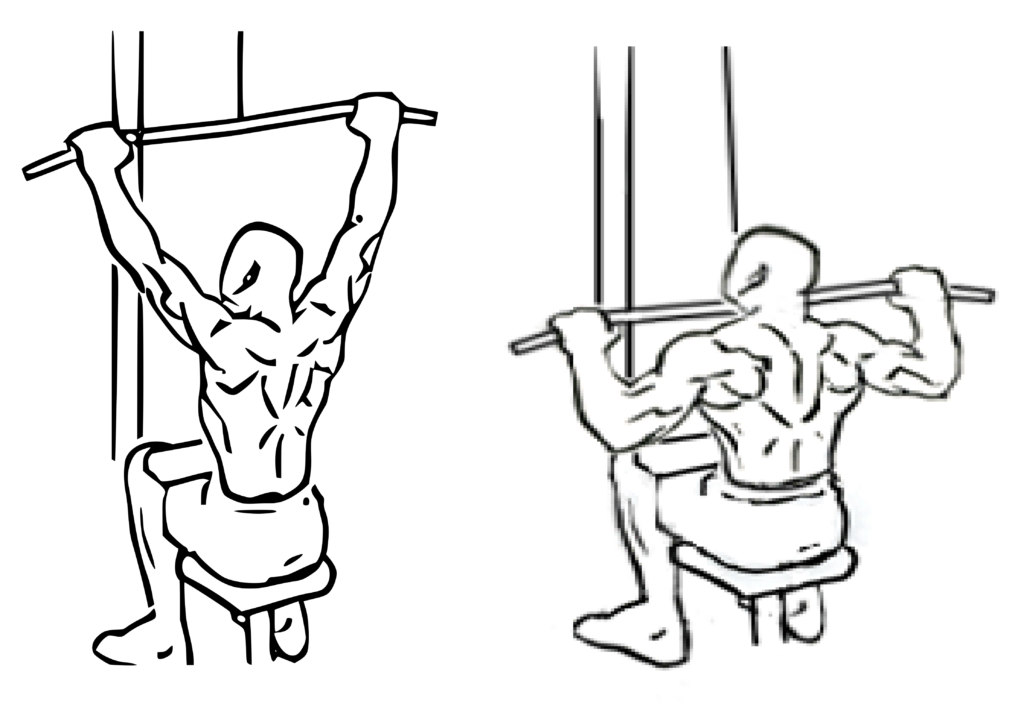
\includegraphics[width=\linewidth, height=60mm]{day_A_ex_1_Wide_grip_lat_pull_down_2-1024x704.png}\end{minipage}&
\begin{minipage}{5cm} 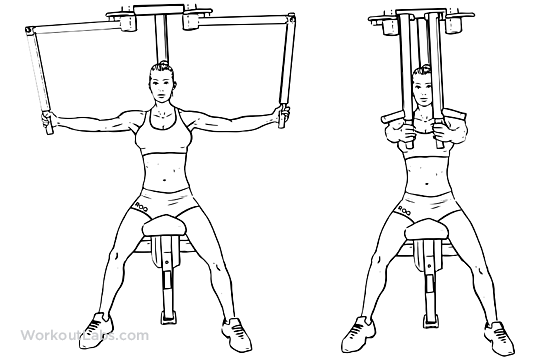
\includegraphics[width=\linewidth, height=60mm]{day_A_ex_2_Butterfly_F_WorkoutLabs.png} \end{minipage}& 
\begin{minipage}{5cm} 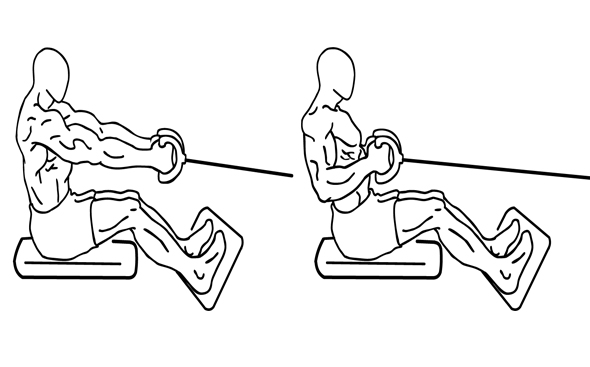
\includegraphics[width=\linewidth, height=60mm]{day_A_ex_3_nab_seated_cable_row.jpg} \end{minipage}\\ 
3-4 х 5-10 reps &  2-4 х 10 &  3-4 х 5-10 reps \\
\hline
4. Повдигане на ръце напред & 5. Повдигане на ръце встрани & 6. Бек екстензии \\ 
\begin{minipage}{5cm} 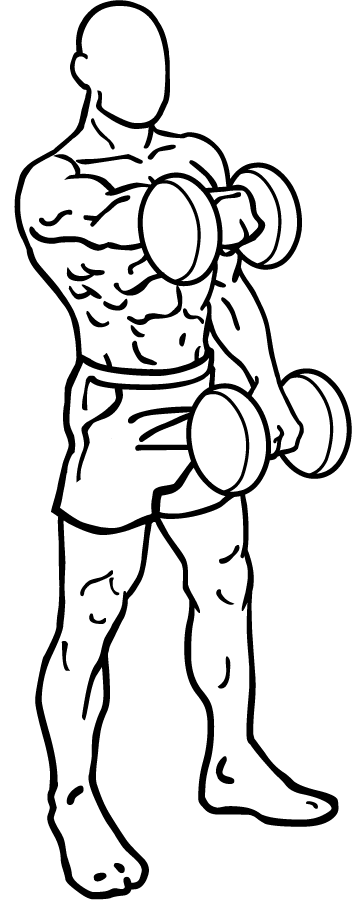
\includegraphics[width=\linewidth, height=60mm]{day_A_ex_5_Dumbbell-front-raises-2-1-1.png} \end{minipage} & 
\begin{minipage}{5cm} 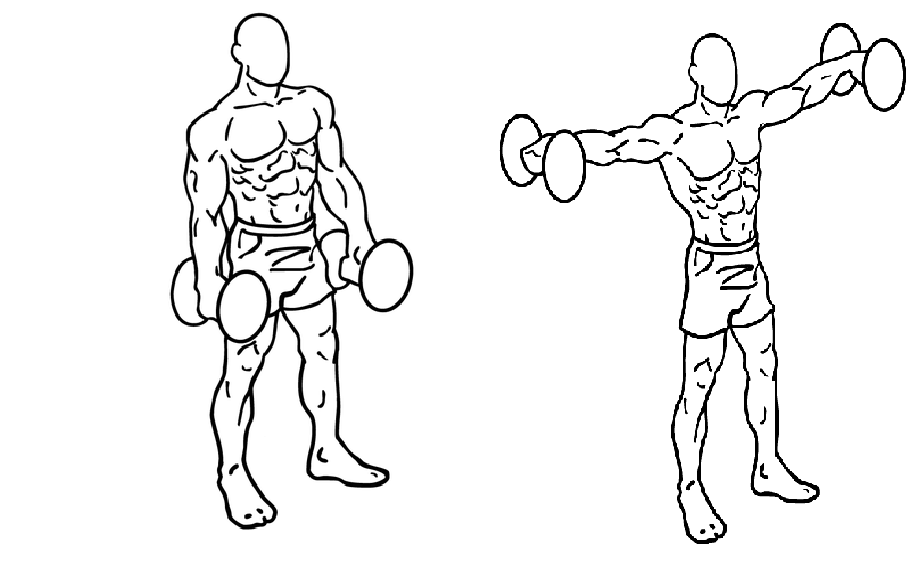
\includegraphics[width=\linewidth, height=60mm]{day_A_ex_6_Dumbbell-lateral-raises-2.png} \end{minipage} &
\begin{minipage}{5cm} 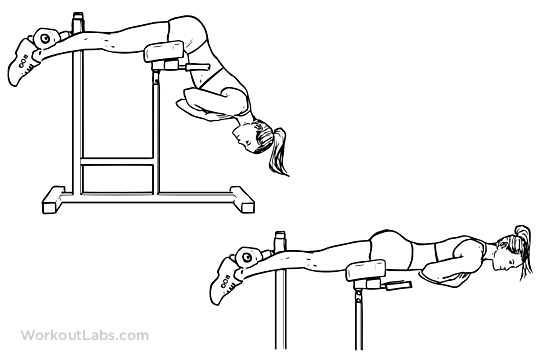
\includegraphics[width=\linewidth, height=60mm]{day_A_ex_4_Back_Extensions.png} \end{minipage} \\
2-3 х 8-10 reps & 2-3 х 8-10 reps & 3-4 х 12-20 reps \\ 
\hline
7. Сгъване на тренажор за коремна мускулатура  & 7. Повдигане на краката от стенд & 8. Кардио \\ 
\begin{minipage}{5cm} 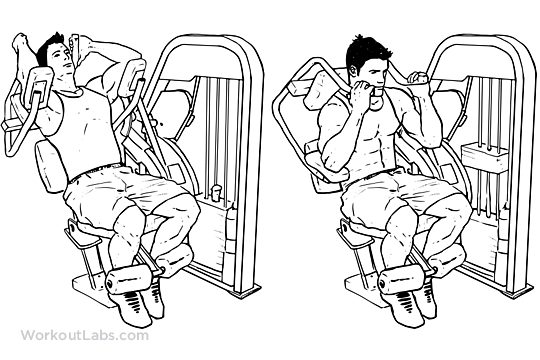
\includegraphics[width=\linewidth, height=60mm]{day_A_ex_7_Ab_Crunch_Machine1.png} \end{minipage} &
\begin{minipage}{5cm} 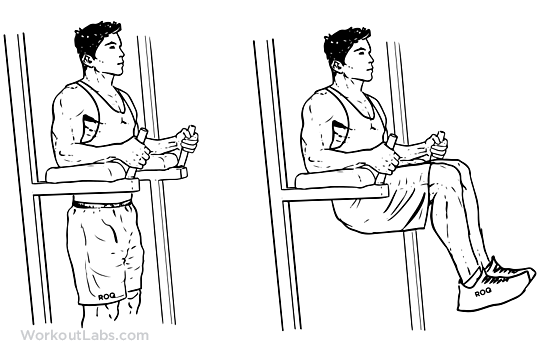
\includegraphics[width=\linewidth, height=60mm]{day_A_ex_7_Knee_Hip_Raise.png} \end{minipage} & 
\begin{minipage}{5cm} 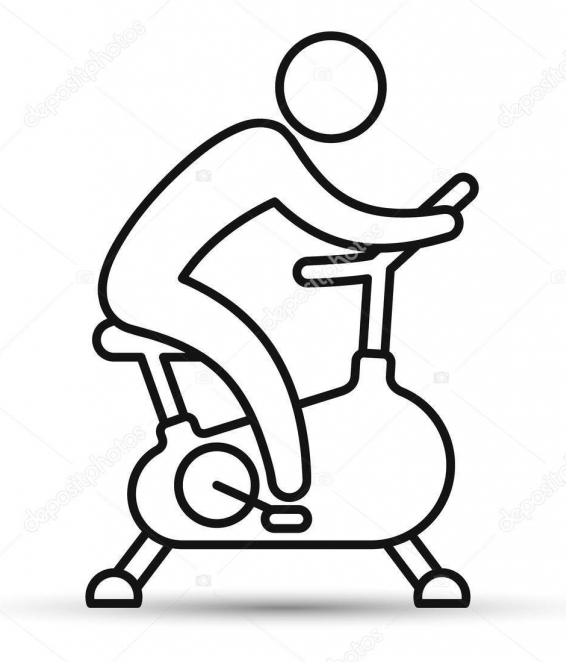
\includegraphics[width=\linewidth, height=60mm]{day_A_ex_8_cardio.jpg} \end{minipage} \\
3-4 х 20-30 reps & 3-4 x 10-20 reps & ~20 (до 40) минути \\ 
\hline
\end{tabular}
\newpage
\textbf{Ден В: доминация на бутащи движения}\\
Загрявка 5 мин. кардио + 2 мин. развъртане на стави (лакти, китки, рамене ,
раменен пояс, таз, колене, глезени, кръст)\\
Загряващи серии 1 х 12-15 за всяко първо движение за мускулна група с малка
тежест\\
Групи: 1+2; 3+4+5; 6+7; 8; 9\\ 
\begin{tabular}{ | m{5cm} | m{5cm} | m{5cm} | }
\hline
1. Избутване на тренажор за гръдна мускулатура & 
2. Високо придърпване хоризонтален скрипец с надхват (дърпа се към брадата)& 
3. Лицеви опори без акцент \\ 
\begin{minipage}{5cm} 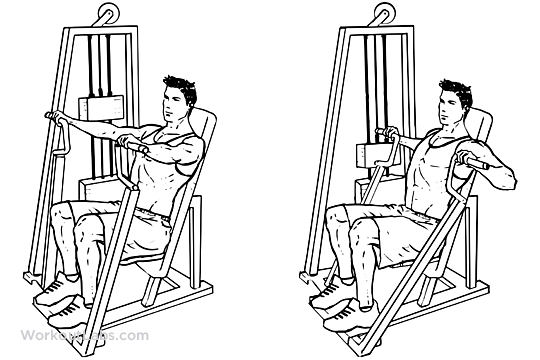
\includegraphics[width=\linewidth, height=60mm]{day_B_ex_1_Hammer_Strength_Machine_Chest_Press_M_WorkoutLabs.png} \end{minipage}&
\begin{minipage}{5cm} 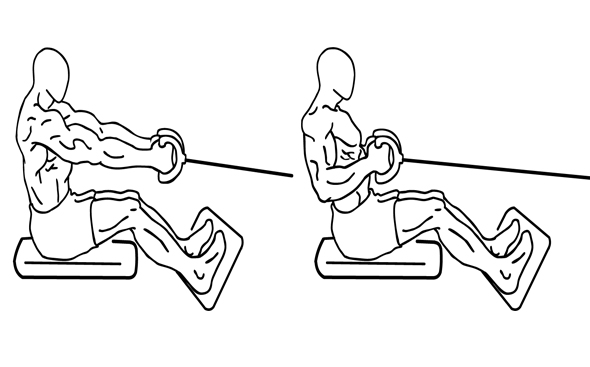
\includegraphics[width=\linewidth, height=60mm]{day_B_ex_2_nab_seated_cable_row.jpg} \end{minipage}& 
\begin{minipage}{5cm} 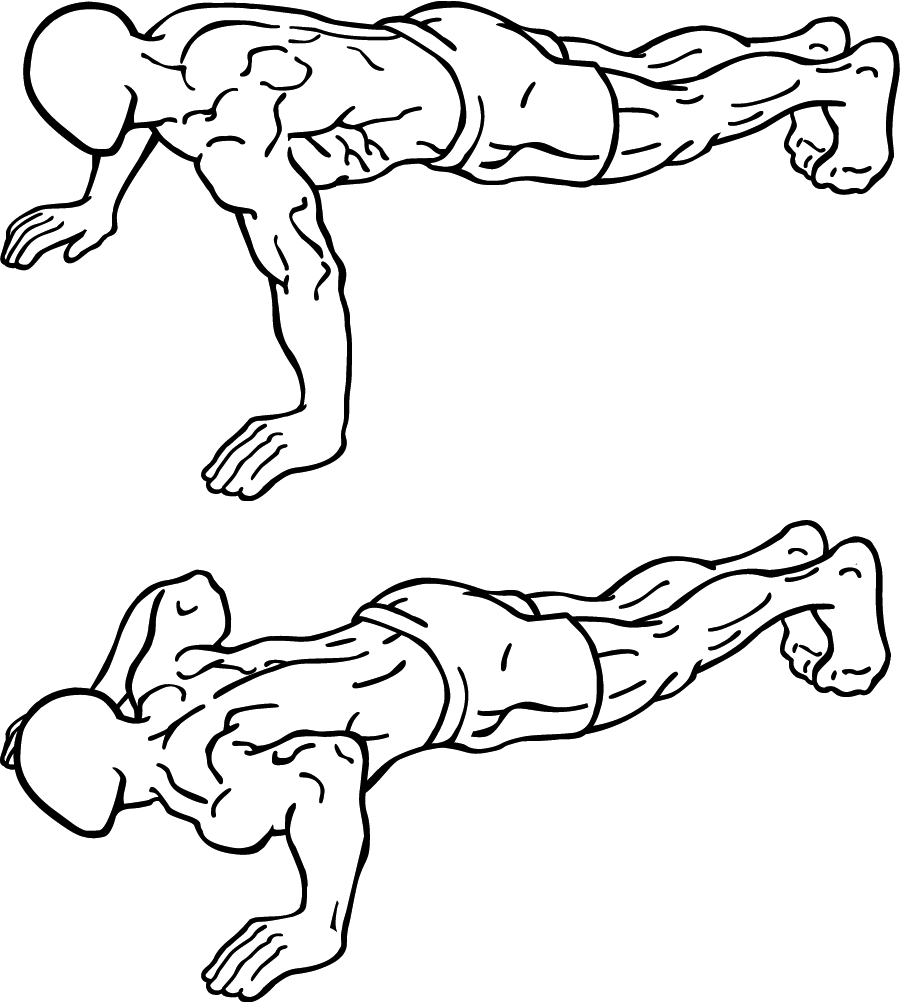
\includegraphics[width=\linewidth, height=60mm]{day_B_ex_3_push-up.png} \end{minipage}\\ 
3-4 х 5-10 reps &   2-3 х 10-12 reps &  3-4 х 5-10 reps \\
\hline
4. Раменни преси на машина & 
5. Пул-даун с прави ръце на горен скрипец/машина & 
6. Чуково сгъване с дъмбели от стоеж  \\ 
\begin{minipage}{5cm} 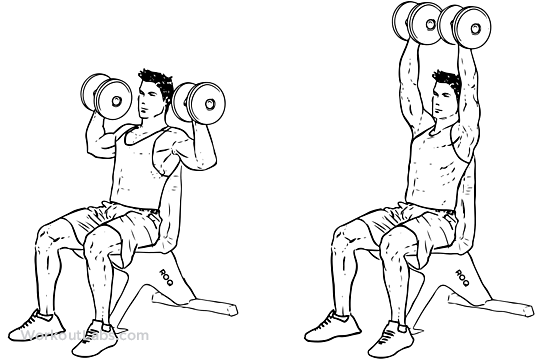
\includegraphics[width=\linewidth, height=60mm]{day_B_ex_4_Dumbbell_Shoulder_Press.png} \end{minipage} &
\begin{minipage}{5cm} 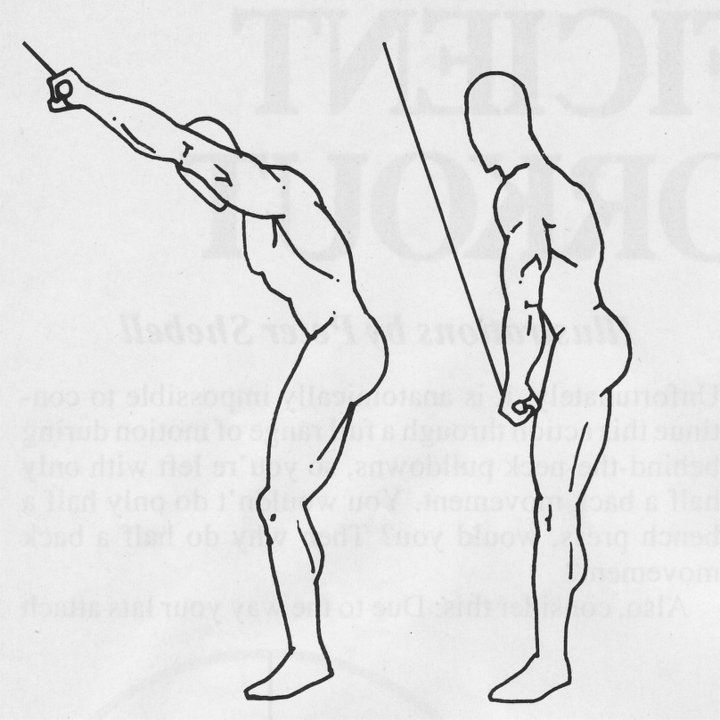
\includegraphics[width=\linewidth, height=60mm]{day_B_ex_5.jpg} \end{minipage} & 
\begin{minipage}{5cm} 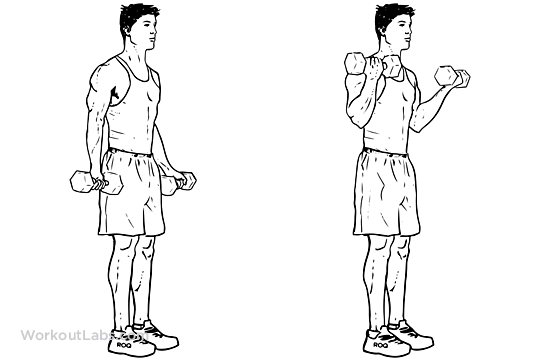
\includegraphics[width=\linewidth, height=60mm]{day_B_ex_6_standing_dumbbell_curl.png} \end{minipage} \\
3-4 х 5-10 reps &  2-3 х 10-12 reps & 2-3 х 5-10 reps \\ 
\hline
7. Разгъване на горен скрипец & 
8. Крънчове (къси коремни сгъвания) ляво-дясно на земя или на пейка& 
9. Кардио \\ 
\begin{minipage}{5cm} 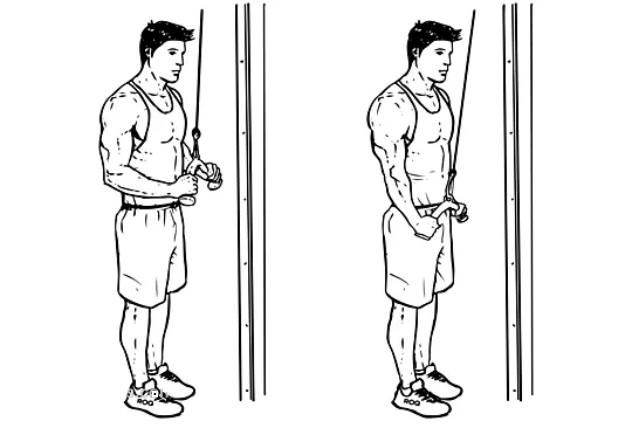
\includegraphics[width=\linewidth, height=60mm]{day_B_ex_7_Standing-Cable-Pushdown.jpg} \end{minipage} &
\begin{minipage}{5cm} 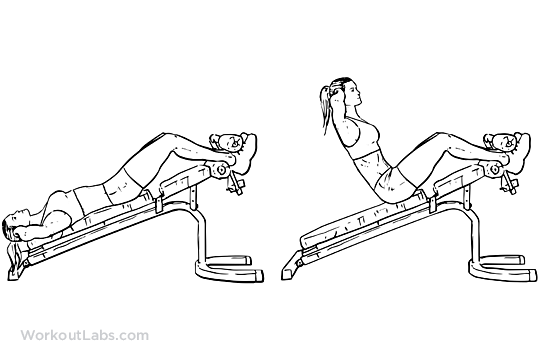
\includegraphics[width=\linewidth, height=60mm]{day_B_ex_8_Decline_Bench_Crunches_Sit-ups_Situps-1.png} \end{minipage} & 
\begin{minipage}{5cm} 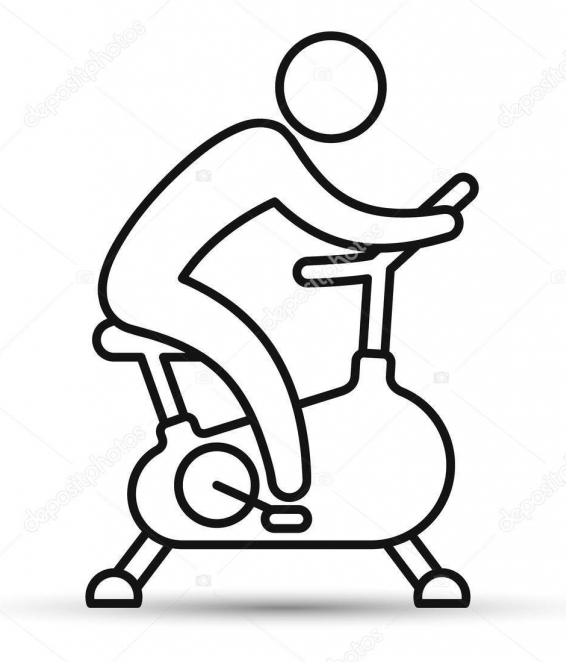
\includegraphics[width=\linewidth, height=60mm]{day_B_ex_9_cardio.jpg} \end{minipage} \\
3-4 х 20-30 reps &  2-4 х 20-30 двойни & ~20 (до 40) минути \\ 
\hline
\end{tabular}


\newpage
\textbf{Ден С: седалищна, бедрена мускулатура и коремен пояс}\\
Загрявка 5 мин. кардио + 2 мин. развъртане на стави (лакти, китки, рамене ,
раменен пояс, таз, колене, глезени, кръст)\\
Загряващи серии 1 х 12-15 за всяко първо движение за мускулна група с малка
тежест\\
Групи: 1+2; 3+4+5;6+7;\\ 
\begin{tabular}{ | m{5cm} | m{5cm} | m{5cm} | }
\hline
1. Полуклек до пейка със собствено тегло & 
2. Преден планк   & 
3  Добро утро с прави крака и диск/дъмбели\\ 
\begin{minipage}{5cm} 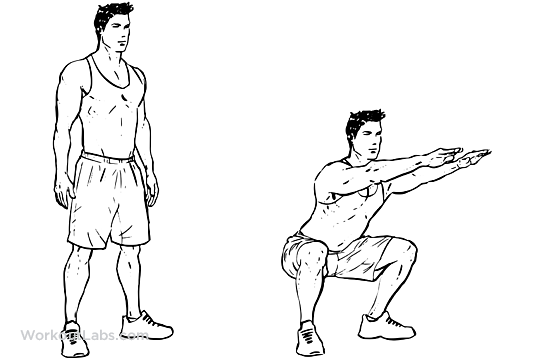
\includegraphics[width=\linewidth, height=60mm]{day_C_ex_1_Air_Squats.png} \end{minipage}&
\begin{minipage}{5cm} 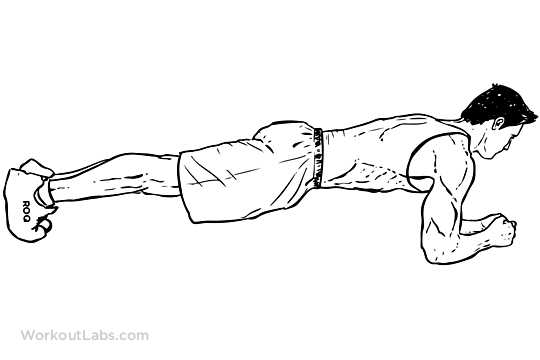
\includegraphics[width=\linewidth, height=60mm]{day_C_ex_2_front-plank.png} \end{minipage}& 
\begin{minipage}{5cm} 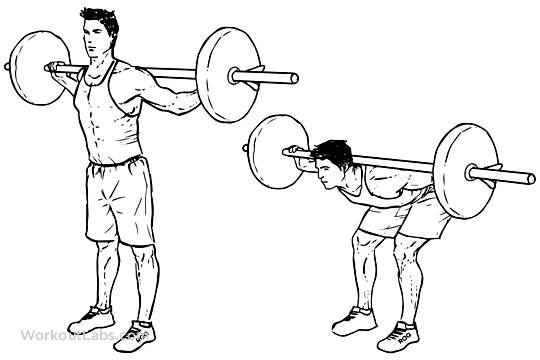
\includegraphics[width=\linewidth, height=60mm]{day_C_ex_3_Barbell_Good_Morning.png} \end{minipage}\\ 
3-4 х 15-30 reps &  2-3 х 40-90 сек &  2-3 х 12-20 reps \\
\hline
4. Страничен планк  & 
5. Катерач (облегнати на пейка) & 
6. Абдуктор машина \\ 
\begin{minipage}{5cm} 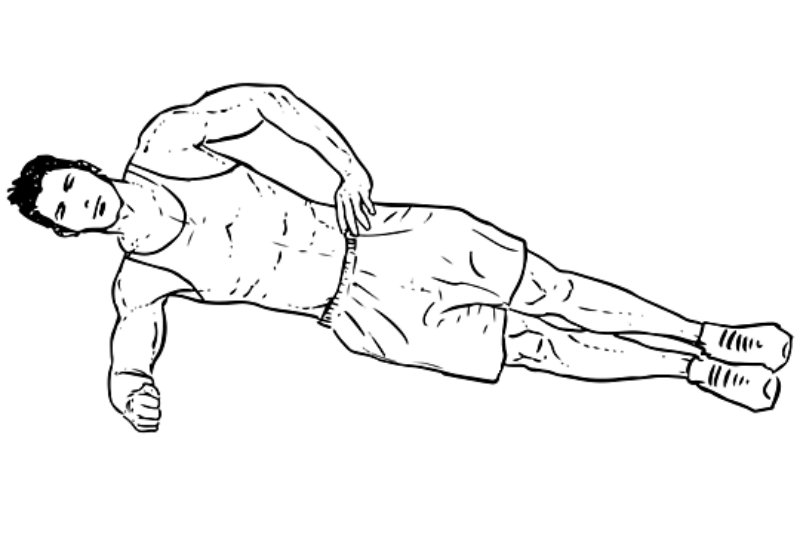
\includegraphics[width=\linewidth, height=60mm]{day_C_ex_4_Side-Plank.png} \end{minipage} &
\begin{minipage}{5cm} 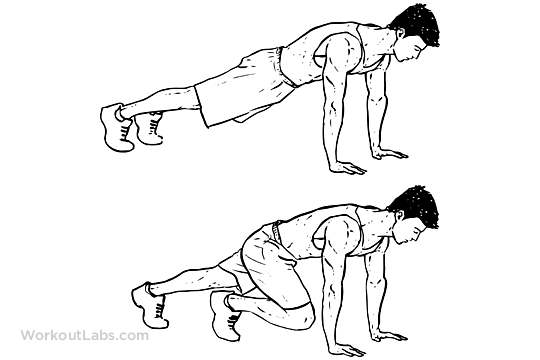
\includegraphics[width=\linewidth, height=60mm]{day_C_ex_5_Mountain_Climbers.png} \end{minipage} & 
\begin{minipage}{5cm} 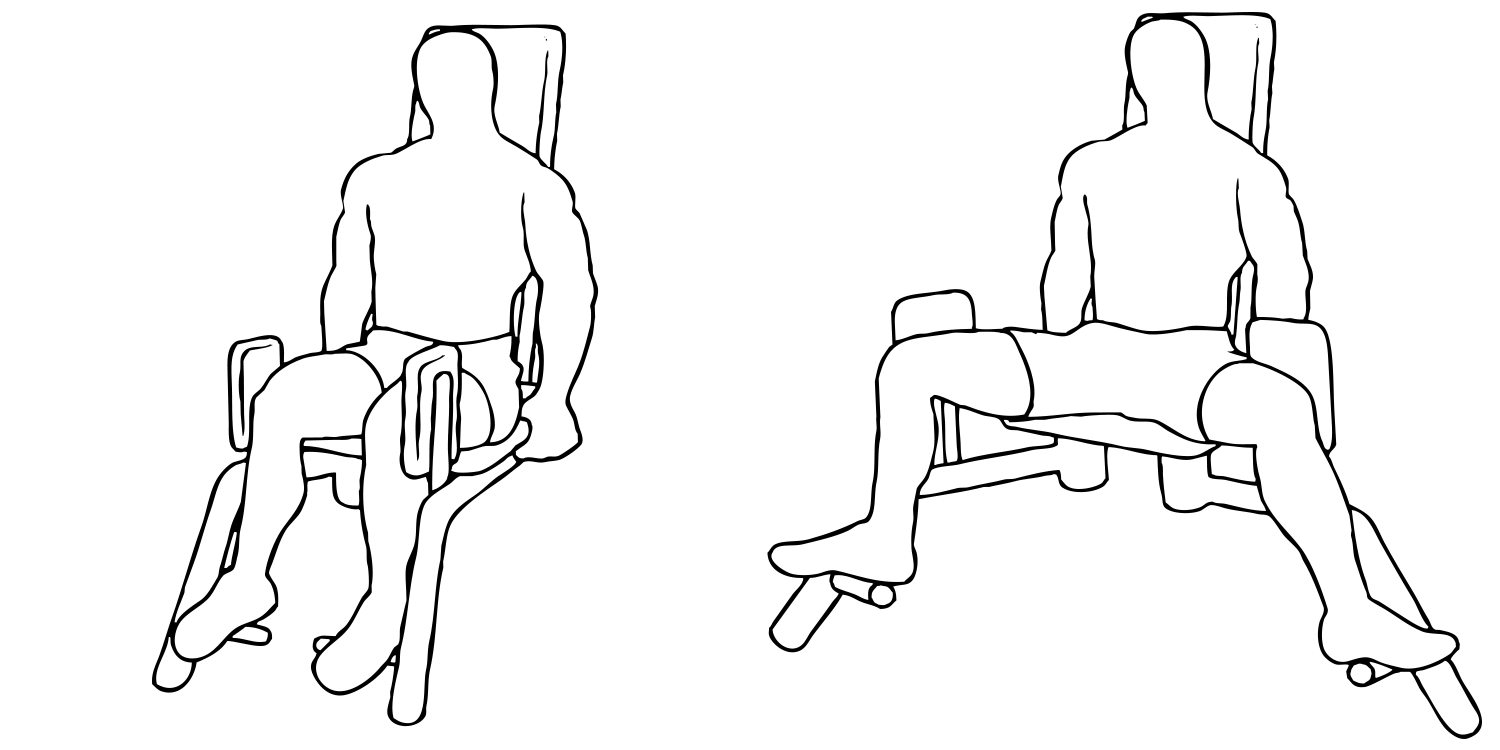
\includegraphics[width=\linewidth, height=60mm]{day_C_ex_6_winner-thigh-abductor.png} \end{minipage} \\
2-3 х 30-60 сек вляво и вдясно & 2-3 х 30 странично + 30 фронтално & 2 х 30-50 Отваряне + 30-50 Затваряне \\ 
\hline
7. Руско извиване (наклона варира според теглото на атлета)& 
8. Задна опора & 
9. Кардио\\ 
\begin{minipage}{5cm} 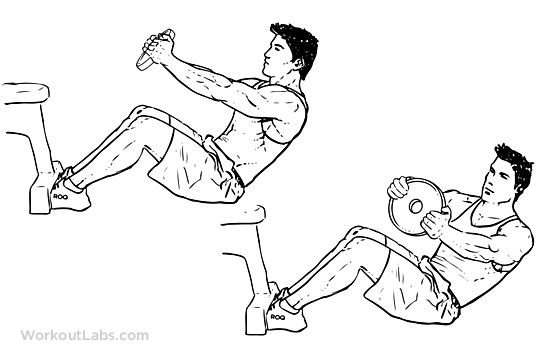
\includegraphics[width=\linewidth, height=60mm]{day_C_ex_7_Russian_Twist.png} \end{minipage} &
\begin{minipage}{5cm} 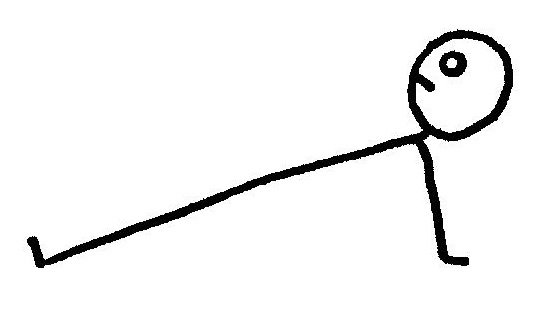
\includegraphics[width=\linewidth, height=60mm]{day_C_ex_8_reverse-plank.jpg} \end{minipage} & 
\begin{minipage}{5cm} 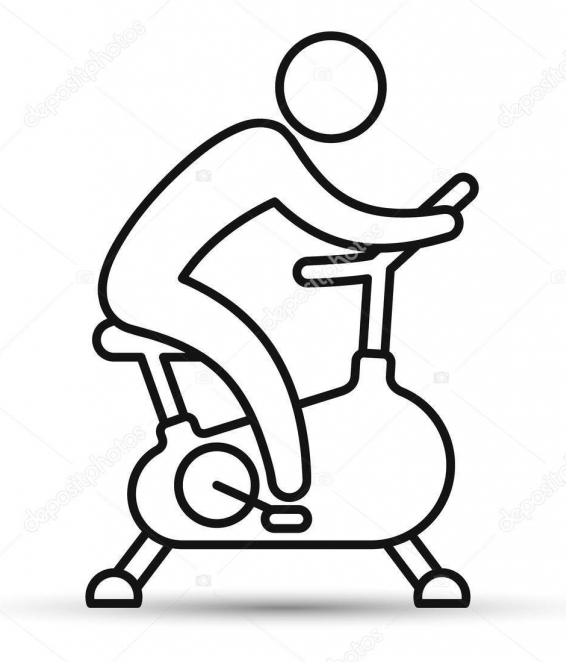
\includegraphics[width=\linewidth, height=60mm]{day_C_ex_9_cardio.jpg} \end{minipage} \\
2 х 20-30 с 2-3 сек. въртене в посока;& 2 х 30-60 сек & ~20 (до 40) минути \\ 
\hline
\end{tabular}

\end{document}
